\documentclass{article}

\usepackage{amsmath,amssymb}
\usepackage{geometry}
\usepackage{graphicx}

\geometry{a4paper, margin=2.5cm}

\begin{document}

% ============================================================
\section*{Model-Based RL: from Environment Models to Dyna-Q}

\subsection*{First, a story}

A traveler arrives in an unfamiliar city. The most direct approach is to memorize each step's outcome: heading north from here --- what feedback, where did I end up; on the next visit to the same spot, repeat the same update. That is the model-free approach. But once the traveler has gradually learned the city map, there is no need to physically walk: on the map one can imagine ``if I go north, where do I land; turning east there, what happens''.

\textbf{The model-free way}: update the value function only with transitions from real interaction.

\textbf{This chapter's way}: learn an environment model from real experience while sampling imagined experience from the model for extra value updates.

\textbf{The core question}: when real interaction is expensive, how do we plan reliably with a learned model?

\[
\boxed{\text{one real interaction} \;\longrightarrow\; \text{update model and }Q \;\longrightarrow\; \text{perform }n\text{ imagined updates}}
\]

Planning does not create information from nothing: state--action pairs the model has never seen still cannot be reliably imagined. The key to Dyna-Q is therefore not merely ``update more often'' but clearly separating real data, model error, and planning compute.

\subsection*{Formalization}

The environment is an MDP: states $s\in\mathcal S$, actions $a\in\mathcal A$, reward $r$, termination flag $d$, and discount $\gamma$. This chapter stays in the finite, fully observable, stationary tabular MDP: state IDs are known, transitions are Markov, and the model only needs to estimate the outcome distribution over $\mathcal S\times\mathcal A$. This restriction splits the problem: first study how planning is affected by model quality, then discuss representation error of neural world models. The model-free Q-learning target is

\[
 y=r+\gamma(1-d)\max_{a'}Q(s',a'),\qquad
 Q(s,a)\leftarrow Q(s,a)+\alpha\bigl(y-Q(s,a)\bigr).
\]

The model is not a single ``next-state table'' but an estimate of the joint outcome:

\[
\boxed{\hat p(s',r,d\mid s,a)}.
\]

It may be deterministic, or store multiple outcomes' frequencies to express the transition distribution of a stochastic environment. When planning, sample $\hat s',\hat r,\hat d$ from $\hat p$ to get

\[
\hat y=\hat r+\gamma(1-\hat d)\max_{a'}Q(\hat s',a').
\]

Let $T$ be the true Bellman optimality operator and $\hat T$ the model operator:

\[
(TQ)(s,a)=\mathbb E_p[r+\gamma(1-d)\max_{a'}Q(s',a')],
\]
\[
(\hat TQ)(s,a)=\mathbb E_{\hat p}[r+\gamma(1-d)\max_{a'}Q(s',a')].
\]

If rewards are bounded $|r|\le R_{\max}$ and $V_Q=\max_{s,a}|Q(s,a)|$, then applying $|\mathbb E_{\hat p}f-\mathbb E_pf|\le(\sup f-\inf f)\cdot\mathrm{TV}$ to $f=(1-d)\max_{a'}Q(s',a')\in[-V_Q,V_Q]$:

\[
\bigl|(\hat TQ-TQ)(s,a)\bigr|
\le |\mathbb E_{\hat p}r-\mathbb E_pr|
+2\gamma V_Q\,\mathrm{TV}\!\left(\hat p,p\right).
\]

This inequality gives the chapter's central claim: model error enters the target at every backup; the bias of $k$ consecutive model backups propagates geometrically. More planning updates pay off only when the statistical error they remove exceeds the model error they propagate.

\begin{itemize}
  \item $\alpha$ is the value-update step size;
  \item $d=1$ marks a terminal state, after which no bootstrap happens;
  \item $n$ is the number of planning updates per real interaction, not extra environment samples.
\end{itemize}

% ============================================================
\section*{Why models and planning}

\subsection*{Sample efficiency and compute budgets}

In real robots, online services or expensive simulators, obtaining a new transition can cost far more than computing one Q update. Under a fixed interaction budget, a model lets one real transition inform many already-observed state--action pairs, propagating reward information faster.

But report both budgets: real environment steps and imagined planning steps. Plotting only total updates easily mislabels planning compute as sample efficiency. With $n=0$, Dyna-Q degenerates to plain Q-learning; with $n>0$, what is added is model-generated updates, not new information.

\subsection*{Model learning and the unknown}

Whenever a real transition $(s,a,r,s',d)$ arrives, the model updates:

\[
\hat p_{t+1}(\cdot\mid s,a)\leftarrow
\operatorname{update}\bigl(\hat p_t(\cdot\mid s,a),(s',r,d)\bigr).
\]

Planning may only sample from the set $\mathcal K$ of already-observed state--action pairs. Mistaking unvisited pairs for ``zero reward and stay in place'' hands the algorithm a fictitious map; the unknown must remain explicitly unknown rather than being quietly filled with a default answer.

\begin{figure}[!htbp]
  \centering
  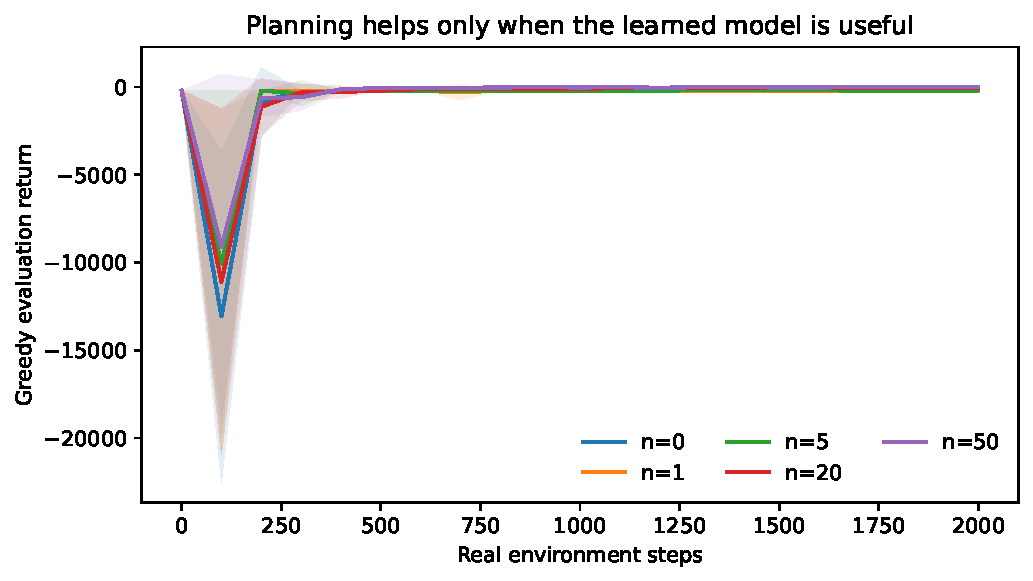
\includegraphics[width=0.88\textwidth]{fig1_sample_efficiency.pdf}
  \caption{Fixed-real-step evaluation curves for different planning budgets $n$ on CliffWalking-v0; the mean and shading come from greedy evaluation over 20 seeds. The x-axis is environment steps, not episode index, so differing episode lengths cannot shift the comparison.}
  \label{fig:dyna-sample-efficiency}
\end{figure}

% ============================================================
\section*{Dyna-Q's core mechanisms}

\subsection*{Real and imagined updates}

Dyna-Q puts both paths in one loop. The real update consumes the transition just returned by the environment, correcting both the model and Q; the imagined update draws previously seen state--action pairs from the model, correcting only Q.

\[
\boxed{
\begin{aligned}
\delta_{\mathrm{real}}&=r+\gamma(1-d)\max_{a'}Q(s',a')-Q(s,a),\\
\delta_{\mathrm{plan}}&=\hat r+\gamma(1-\hat d)\max_{a'}Q(\hat s',a')-Q(\hat s,\hat a).
\end{aligned}}
\]

Both use the same Q-update form but differ in information source. The real update corrects; the planning update propagates. If the model is systematically biased, planning amplifies that bias systematically.

\subsection*{The meaning of the planning count $n$}

After each environment step: first the real update, then draw $n$ state--action pairs uniformly from $\mathcal K$. Larger $n$ means more compute per real interaction; with an accurate model this usually speeds learning; with a stale or wrong model it can breed overconfidence.

\begin{figure}[!htbp]
  \centering
  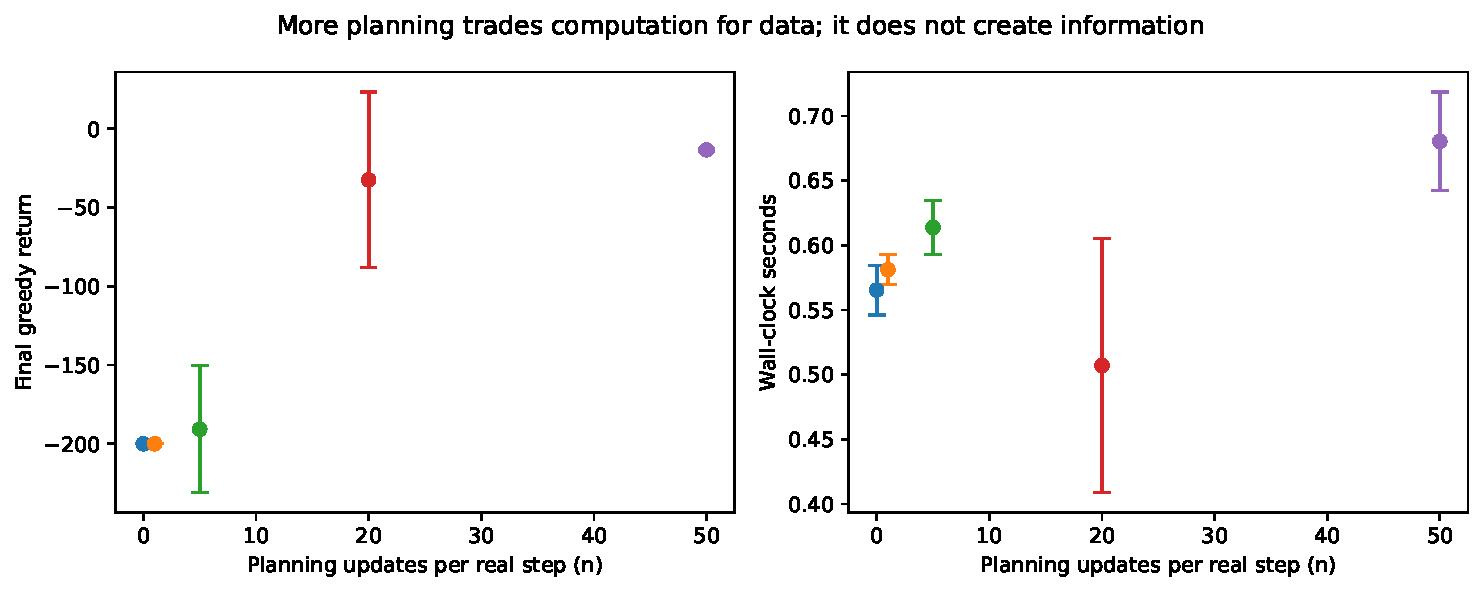
\includegraphics[width=0.88\textwidth]{fig2_planning_sweep.pdf}
  \caption{Final greedy return and wall-clock time after the same 2000 real environment steps; 20 seeds per $n$. The left panel measures data efficiency; the right shows the extra compute cost of planning --- simulated updates are not counted as new samples.}
  \label{fig:dyna-planning-sweep}
\end{figure}

\subsection*{Planning count $n$ is not planning depth}

Our Dyna-Q performs a single model backup per planning step. $n$ counts backups, not the depth of imagined trajectories: when a reward change in the model must propagate through several predecessor states, those states must be drawn repeatedly. The alternative is rolling out a length-$H$ model trajectory from the current state, constructing

\[
\hat G_H=\sum_{j=0}^{H-1}\gamma^j\hat r_j+\gamma^H\max_a Q(\hat s_H,a).
\]

This is not equivalent to $n=H$ Dyna updates: the former absorbs model error continuously along one imagined trajectory; the latter spreads a bounded number of backups over many state--action pairs. As $H$ grows, local transition errors compose over many steps; growing $n$ mainly changes compute allocation.

\subsection*{Priority: why uniform sampling is not always right}

Uniform planning treats every observed pair as equally important, but a reward change often affects only a small region of predecessors. Prioritized Sweeping maintains for each candidate backup the priority

\[
p(s,a)=\left|\hat r+\gamma(1-\hat d)\max_{a'}Q(\hat s',a')-Q(s,a)\right|,
\]

each time updating the highest-priority pair and enqueueing its model predecessors. Value changes then propagate quickly backwards along the predecessor graph; the cost is maintaining predecessors and a queue, and high priority does not mean high model trust. Priority solves \textbf{compute allocation}, not exploratory uncertainty: $\epsilon$-greedy decides where to collect real data; confidence upper bounds or uncertainty bonuses are a different family of designs that actively exploit model uncertainty.

\subsection*{Model bias in stochastic environments: a reproducible failure mode}

In stochastic environments like FrozenLake one $(s,a)$ can lead to several successors. A deterministic model storing only the last observation misreads randomness as determinism; storing empirical frequencies expresses uncertainty but still has variance under insufficient data. The benefit of planning depends on model error, visit coverage, and the planning budget jointly.

Consider a two-state counterexample: action $a$ yields $0$ with probability $0.99$ and transitions with probability $0.01$ to a state with reward $+100$. If the last finite sample happened to be $0$, the last-observation model undervalues the action; if it happened to be the rare $+100$, heavy planning turns one accident into a certainty. The larger $n$, the more often the wrong model is reused. The empirical distribution converges as samples grow, but under thin coverage it too must not be mistaken for the true kernel. The counterexample shows: planning can save interaction but cannot replace information gathering.

\begin{figure}[!htbp]
  \centering
  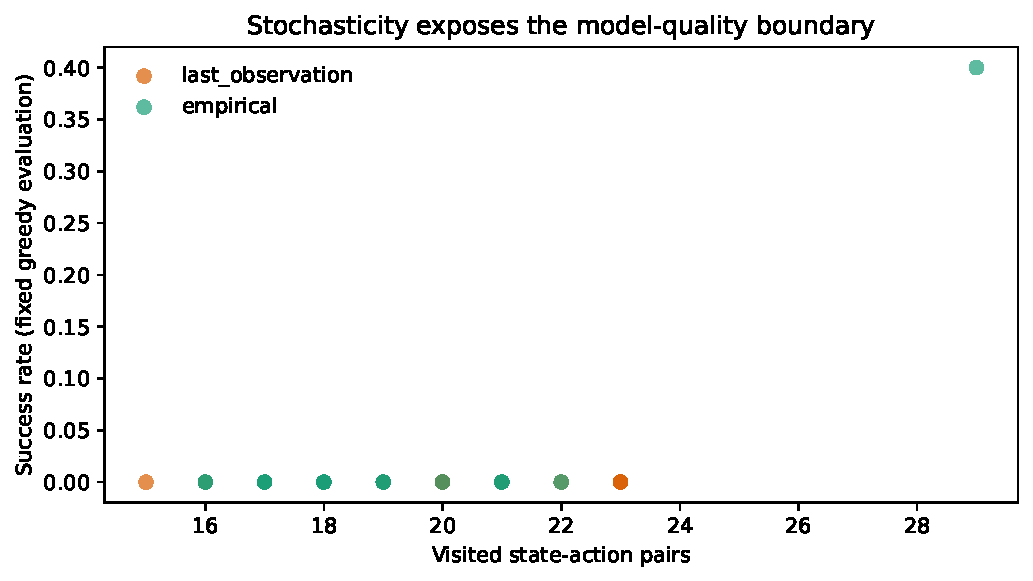
\includegraphics[width=0.88\textwidth]{fig3_model_bias.pdf}
  \caption{Coverage--success-rate diagnostics for last-observation vs.\ empirical models on stochastic FrozenLake-v1; each point is one seed, success rates from a fixed, exploration-free greedy evaluation. The figure compares model representations and does not inflate correlation into causation.}
  \label{fig:dyna-model-bias}
\end{figure}

On deterministic CliffWalking, once the model has observed the outcome of $(s,a)$ it can replay it exactly; on stochastic FrozenLake the model must also estimate an outcome distribution. To avoid conflating the two error types, experiments should report separately: observed state--action coverage, the model's transition-prediction error, real environment steps, planning backups, and returns or success rates under a fixed evaluation protocol. The scatter in Figure~3 is a diagnostic relation, not causal proof; alone it cannot establish ``uncertainty causes lower returns''.

\subsection*{The algorithm}

\begin{enumerate}
  \item \textbf{Initialize}: $Q(s,a)=0$, model empty, observed set $\mathcal K=\varnothing$;
  \item \textbf{Act}: choose $a$ $\epsilon$-greedily from the current $Q$; the environment returns $(s',r,d)$;
  \item \textbf{Real Q update}: update $Q(s,a)$ with $r+\gamma(1-d)\max_{a'}Q(s',a')$;
  \item \textbf{Model update}: write $(s',r,d)$ into $\hat p(\cdot\mid s,a)$ and add $(s,a)$ to $\mathcal K$;
  \item \textbf{Planning loop}: for $i=1,\ldots,n$, sample $(\hat s,\hat a)$ from $\mathcal K$, sample $(\hat s',\hat r,\hat d)$ from the model, and perform one imagined Q update;
  \item \textbf{Continue}: reset if terminal, else $s\leftarrow s'$.
\end{enumerate}

The order matters: write real experience into the model \emph{before} letting planning use it. Planning first would delay the new information by one cycle.

\subsection*{Comparison with neighbors}

\begin{itemize}
  \item \textbf{Q-learning}: $n=0$; only real transitions update the value;
  \item \textbf{Dyna-Q}: learns an explicit model and plans from it;
  \item \textbf{Dynamic programming}: assumes a known model and backs it up systematically;
  \item \textbf{Model-predictive control}: typically replans online and executes short action sequences, not necessarily maintaining a long-term Q;
  \item \textbf{Modern latent planning}: MuZero, Dreamer and kin roll out in learned latent spaces but face the same model bias and coverage issues.
\end{itemize}

% ============================================================
\section*{Where this chapter sits in the RL landscape}

\begin{enumerate}
  \item \textbf{Upstream}: MDPs, TD learning and Q-learning supply the value backup;
  \item \underline{\textbf{Dyna-Q}}: learn an environment model; update values with both real and imagined experience;
  \item \textbf{Downstream}: model-predictive control, latent world models, MuZero, and offline RL with model rollouts.
\end{enumerate}

The chapter's most important conclusion: model-based RL is not simply ``model-free methods plus a predictor'' but a layered system of information sources. Real interaction brings new information; the model reuses it; planning propagates it --- all three must be measured separately in experiments. The natural next steps follow model error and long rollouts: stronger world models and uncertainty estimation.

\subsection*{References}

\begin{enumerate}
  \item Sutton, R. S. (1991). Dyna, an integrated architecture for learning, planning, and reacting. \textit{ACM SIGART Bulletin}.
  \item Sutton \& Barto (2018). \textit{Reinforcement Learning: An Introduction} (2nd ed.). Chapter~9.
  \item Schrittwieser et al. (2020). Mastering Atari, Go, chess and shogi by planning with a learned model. \textit{Nature}.
\end{enumerate}

\end{document}
